\section{Commande de systèmes multi-agents}

Il existe différentes stratégies de contrôle permettant de gérer ces essaims en fonction des contraintes et des objectifs du système.
Deux grandes approches existent pour le contrôle des essaims de robots : le contrôle centralisé et le contrôle décentralisé \cite{jamshidpey_centralization_2024}.

Dans un système centralisé, un ordinateur central connaît la position de chaque robot et leur envoie des commandes pour atteindre une formation donnée. Dans un système décentralisé, chaque robot prend des décisions localement en fonction de son environnement et des autres robots. Dans le cadre du projet eSWARM, les deux approches sont réalisables, à condition de pouvoir faire tourner des programmes plus ou moins complexes directement sur les modules du système.

\begin{table}[h]
    \centering
    \resizebox{\columnwidth}{!}{
    \begin{tabular}{|c|p{6cm}|p{6cm}|}
        \hline
        \textbf{Approche} & \textbf{Avantages} & \textbf{Inconvénients} \\
        \hline
        Contrôle centralisé & Précision, simplification du calcul global & Forte dépendance aux communications \\
        \hline
        Contrôle décentralisé & Robustesse, évolutivité & Coordination plus complexe \\
        \hline
    \end{tabular}}
    \caption{Comparaison du contrôle centralisé et décentralisé \cite{jamshidpey_centralization_2024}}
    \label{tab:comparaison_controle}
\end{table}

\noindent La commande centralisée, étant plus simple à mettre en place, sera mise en œuvre en premier durant le stage, puis un équivalent décentralisé sera développé. 

\subsection{Approches pour le contrôle d’essaim}

Cette section regroupe différentes méthodes utilisées pour le contrôle d'essaim de robot. Comme expliqué précédemment, les premiers algorithmes de contrôle seront développés pour des robots terrestres (section \ref{partie:turtlebot}). \cite{tsiu_survey_2020} est une étude de différentes méthodes de contrôle d'essaim. La partie suivante regroupe donc des algorithmes utilisés pour des systèmes multi-agents.

\subsubsection*{Matrice de distribution}

Une matrice de distribution, comme mentionnée dans la section \ref{partie:aug_bon} du présent rapport, permet de déterminer les commandes à transmettre à chaque module d'un système assemblé de plusieurs modules. Son principal inconvénient réside dans la nécessité de concevoir un moyen automatisé pour générer cette matrice, car elle dépend de la structure formée par les différents modules.

\subsubsection*{Changement de modèle}
\begin{wrapfigure}{r}{0.5\textwidth}
    \vspace{-1cm} 
    \centering
    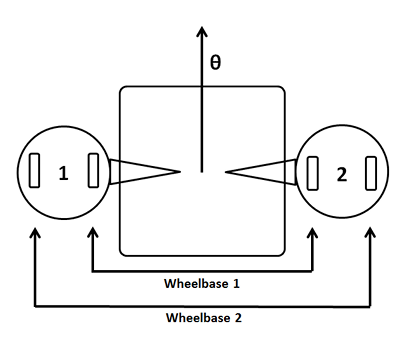
\includegraphics[scale=0.8]{8-Etat_de_art/essaim/pic/changement modele.png}
    \caption{Changement de modèle selon \cite{inglett_object_2017}}
    \label{fig:chgmodl}
    \vspace{-0.3cm} 
\end{wrapfigure}
\cite{inglett_object_2017} décrit un système modulaire composé de plusieurs robots holonomes pouvant s'accrocher entre eux, afin de porter une charge lourde. La solution proposée pour piloter le système est de changer le modèle. Par exemple, deux robots terrestres non holonomes sont accrochés l'un à l'autre horizontalement (voir Figure \ref{fig:chgmodl}), il est possible de considérer les deux roues intérieurs à la structure (Wheelbase 1 sur la Figure \ref{fig:chgmodl}) comme étant un module à piloter (similaire au robot initiale, avec deux roues). De la même manière, les deux roues à l'extérieur forment un deuxième module.
Cette méthode possède plusieurs inconvénients majeurs : 
\begin{itemize}
    \item Il faut être en mesure de pouvoir commander individuellement chaque moteurs du système, ce qui peut être complexe  dans l'optique d'une implémentation avec des drones
    \item Il faut connaître la configuration, et en déterminer le nouveau modèle (c'est-à-dire quels moteurs formeront un module)
    \item Elle nécessite que les différents modules soient attachés physiquement, il n'y a pas d'asservissement de l'inter-distance entre les modules
\end{itemize}

\subsubsection*{Loi de consensus}
La loi de consensus \cite{ali_practical_2018, koung_consensus-based_2020} est une technique de contrôle d'essaim de robots, qui leur permet de se coordonner de manière distribuée. Chaque robot échange des informations avec ses voisins et ajuste son comportement pour atteindre un objectif commun. 

\noindent Dans un système à $n$ robots, on note chaque robot $i$. L'algorithme de consensus classique peut être formulé comme suit :
\begin{equation}
u_i(t) = \sum_{j=1}^{n} a_{ij}(t) [x_j(t) - x_i(t)]
\end{equation}
où $x_i(t)$ est l'état du robot $i$ à l'instant $t$, $u_i(t)$ est l'entrée de contrôle appliquée à ce robot et $a_{ij}(t)$ est l'élément de la matrice d'adjacence qui représente la connexion entre les robots $i$ et $j$. Cette formule signifie que le robot $i$ ajuste son état en fonction de la différence entre son propre état et celui de ses voisins, pondéré par les valeurs de $a_{ij}(t)$.

L'objectif du protocole de consensus est d'amener tous les robots à converger vers un état commun, tel qu'une position ou une vitesse moyenne, indépendamment des différences initiales. Il permet donc de déterminer une consigne pour chaque robot.

\subsubsection*{Méthode Leader-follower}

La méthode leader–follower \cite{loria_leaderfollower_2016, yang_adaptive_2021} est une stratégie de contrôle utilisée dans les systèmes multi-agents, où un ou plusieurs robots appelés leaders définissent la trajectoire ou le comportement à suivre, tandis que les autres robots, appelés followers, ajustent leur mouvement pour maintenir une certaine relation avec ces leaders. Contrairement à la loi de consensus, cette approche introduit une hiérarchie dans l’essaim, ce qui peut simplifier la coordination globale du système.

Dans cette méthode, chaque robot follower $i$ adapte sa position $x_i(t)$ en fonction de la position du leader $x_L(t)$, ou de celle d'autres followers proches, selon le graphe de communication.

\subsubsection*{Asservissement de position du centroïde}

\cite{kloetzer_temporal_2007} présente une méthode hiérarchique pour contrôler automatiquement des essaims en combinant une abstraction continue (centrée sur des caractéristiques globales comme le centroïde et la dispersion du groupe) et une abstraction discrète (reposant sur la logique temporelle linéaire). Cette stratégie permet de spécifier des objectifs, comme atteindre une zone tout en évitant des obstacles, en maintenant la cohésion. La formation du groupe est assurée non pas par un asservissement direct des distances inter-robots, mais en contrôlant globalement la variance des positions. L’approche offre plusieurs avantages, notamment une automatisation complète du processus de planification et une capacité à gérer un grand nombre de robots. Toutefois, elle nécessite un contrôle centralisé.


\subsubsection*{Classification de méthodes de contrôle d'essaim}
\cite{oh_survey_2015} est un article décrivant trois catégories de contrôle d'essaim de robot :
\begin{itemize}
    \item \textit{Contrôle par position : } Chaque robot connaît sa position dans un système de coordonnées global et ajuste activement sa position pour atteindre la formation souhaitée.
    \item \textit{Contrôle basé sur le déplacement : }  Un robot ajuste les déplacements de ses voisins pour atteindre la formation désirée, en supposant qu’il peut mesurer les positions relatives de ses voisins dans le système de coordonnées global, sans pour autant connaître sa propre position absolue.
    \item \textit{Contrôle basé sur la distance : } Les robots ajustent activement les distances inter-agents pour atteindre la formation cible. Ils perçoivent uniquement les positions relatives de leurs voisins dans leur propre référentiel local, sans nécessiter d’alignement des orientations entre les référentiels des différents agents.
\end{itemize}
\vspace{0.3cm}


%-----------------------------------------------------------------------------
% Transition commande évennementielle

\begin{wrapfigure}{r}{0.4\textwidth}
    \vspace{-0.2cm} 
    \centering
    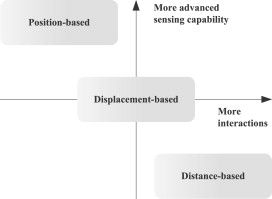
\includegraphics[width=\linewidth]{8-Etat_de_art/essaim/pic/meth_swarm.jpg}
    \caption{Comparaison des méthodes de contrôle \cite{oh_survey_2015}}
    \label{fig:met_swarm}
    \vspace{-3cm} 
\end{wrapfigure}

L'article \cite{oh_survey_2015} fait également mention des avantages et inconvénients de chaque méthode de commande d'essaim, en mettant l'accent sur la complexités de capteur à mettre en place et la quantité de données à transmettre. Par exemple, le contrôle par position nécessite des capteurs plus complexes, mais les échanges de données sont moins nombreux. L'inverse s'applique pour le contrôle basé sur la distance. Il serait donc pertinent d'utiliser une commande évènementielle dans ce cas la afin d'améliorer les performances.

